\documentclass{standalone}
\usepackage{tikz}
\usepackage{ctex,siunitx}
\setCJKmainfont{Noto Serif CJK SC}
\usepackage{tkz-euclide}
\usepackage{amsmath}
\usepackage{wasysym}
\usetikzlibrary{patterns, calc}
\usetikzlibrary {decorations.pathmorphing, decorations.pathreplacing, decorations.shapes,}
\begin{document}
\small
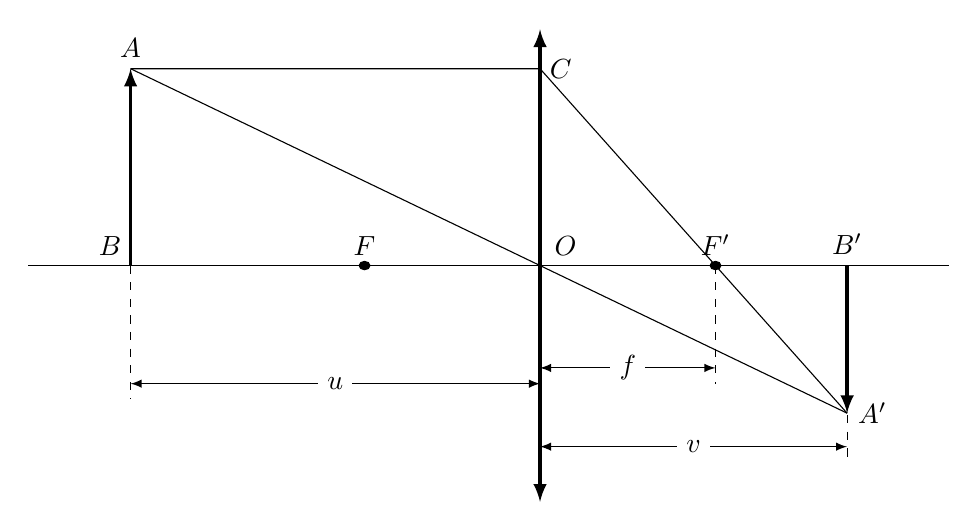
\begin{tikzpicture}[>=latex,xscale=1.3]
  \draw[<->, very thick ] (0,3)--(0,-3);
  \draw (-5,0)--(4,0);
  \draw [->, very thick, >=latex](-4,0)--(-4,2.5)node[above]{$A$};
  \node at (-4-.2,0.25){$B$};
  \draw (-4,2.5)--(0,2.5)node[right]{$C$}--(3,-2.5*.75);
  \draw (-4,2.5)--(0,0)--(3,-2.5*.75);
  \draw [->, very thick, >=latex](3,0)node[above]{$B'$}--(3,-2.5*.75)node[right]{$A'$};
  \draw [dashed](12/7,0)node[above]{$F'$}--(12/7,-1.5);
  \draw[<->,>=latex] (0,-1.3)--node[fill=white]{$f$}(12/7,-1.3);
  \draw[<->,>=latex] (0,-1.5)--node[fill=white]{$u$}(-4,-1.5);
  \draw [dashed](-4,0)--(-4,-1.7);  \draw [dashed](3,0)--(3,-2.5);
  \draw[<->,>=latex] (0,-2.3)--node[fill=white]{$v$}(3,-2.3);
  \node at (0.25,.25){$O$};
  \node at (-12/7,.25){$F$};
  \draw  (12/7,0)[fill=black] circle (1.5pt);
  \draw  (-12/7,0)[fill=black] circle (1.5pt);
\end{tikzpicture}
\end{document}